\chapter{Foundation}

In vessel handling terminology, maneuvering refers to the task of controlling a vessel’s movement using its propulsion and navigation systems; taking into account environmental forces such as wind, waves and, current acting on the vessel. Vessels move in a variety of marine environments. Starting from ports in harbors where the water is shallow and vessel traffic is high, a vessel might navigate the vast open seas to a different port in a harbour across the ocean. Vessels also navigate inland waterways such as rivers, canals, backwaters and creeks. More recently, developments in offshore wind farming and the oil and gas industry have necessitated regular and frequent visits to offshore structures located on continental shelves. Figure \ref{fig:northseamap} shows some prominent offshore oil fields in the North sea. 

\begin{figure}
	\centering
	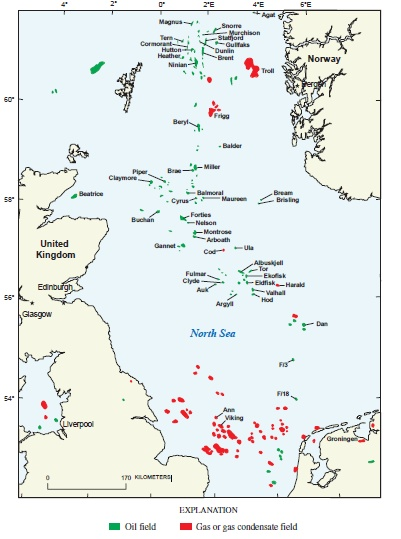
\includegraphics[scale=0.75]{northseaoilandgasmap}
	\caption{Map of oil and gas fields in the North sea}
	%\todo[inline]{Get higher resolution picture}
	\label{fig:northseamap}
\end{figure}

% More recently, offshore wind energy and the oil and gas industry have  offshore structures typically located on continental shelves some miles off the coast. 


%Recently, developments in the oil and gas industry have necessitated extensive use of specialised vessels called offshore supply vessels in aid of exploration and production operations. These 

%the construction and maintenance of offshore oil platforms typically located in continental shelves. 

Handling vessels at low speeds has been difficult on marine vessels historically. From a technical point of view, the working mechanism of rudder systems of the past made it difficult to turn vessels in place. From a human operator perspective, the challenge of maneuvering at low speed is further amplified when the operation occurs in close proximity to large physical objects due to the added stress from the risk of collision. Refer to \cite{inoue2000evaluation} for a method of objective evaluation of ship handling difficulties in restricted maneuvering area or in areas of traffic congestion. Examples of difficult maneuvering operations are approaching a harbour, berthing in a port, sailing side-by-side another vessel, approaching and stationing close to an oil platform, etc. An often recurring sequence is that of  port-bound vessel heading to its berthing location in the harbour. Having entered pilot waters from seaward, a vessel's course needs to be controlled to ensure safe passage through channels, bridges, and locks; while avoiding collisions with other vessels at the same time. Safety risks involved in such tasks make it a stressful operation. Mistakes have high associated costs, possibly leading to lost lives and damage to expensive constructions.


% Mistakes in execution have high costs associated with them as they can lead to lost lives and damage to expensive constructions. 

%Executing a maneuvering operation in close proximity to large man-made physical structures is particularly challenging. the added stress due to risk of collision makes the task particularly challenging. 
%A maneuvering operation that takes place in close prox
\subsection{Offshore Supply Operations}
A special application of ship handling skill is on-board offshore supply vessels. Offshore supply vessels are cargo vessels that regularly transport goods, supplies or equipment in support of exploration or production of offshore mineral or energy resources. Specific missions include: 
\begin{itemize}
\item seismic survey to locate potential oil and gas fields
\item towing of rigs to their location, positioning them and laying anchoring and mooring equipment
\item supplying equipment, personnel, provisions, other necessary goods to rigs
\item subsea operations such as ROV operation, diving support, inspection and maintenance
\item safety standby for emergency response and rescue operations
\end{itemize}
 Offshore supply vessels need to regularly approach and be stationed close to offshore oil platforms to perform supply operations. A platform supply vessel for example, is used to transport supplies such as fuel, water and chemicals to oil platforms; bringing back disposables for proper recycling. 
 
\begin{figure}[h]
	\centering
	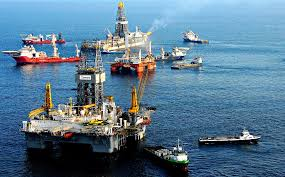
\includegraphics[scale=1.25]{osvbig}
	\caption{Offshore supply vessels in operation}
	\label{fig:shipforces}
\end{figure}

\subsubsection{Dynamic Positioning}

A typical loading operation happens at the stern of the ship. requires station keeping.
This requirement led to the development and subsequent popularity of dynamic positioning systems. Dynamic positioning (DP) is a computer-controlled system that maintains position and heading of a vessel automatically by using its propellers and thrusters. Information from position reference sensors that provide the vessel’s position and heading, along with information from wind sensors, motion sensors and gyrocompasses on the vessel are used by the system. The information is supplied as input to a program that calculates the changes in position/heading required to bring the vessel a preset location and, activates the vessel’s thrusters as necessary.

\begin{figure}
	\centering
	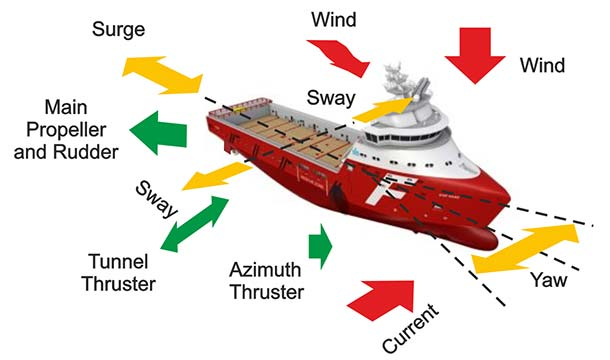
\includegraphics[scale=0.60]{dynamic-positioning}
	\caption{Forces acting on a ship and its possible movements}
	\label{fig:shipforces}
\end{figure}
\todo[inline]{make own picture with legend of forces}
%Write about the popularity of Dp systems, its advantages and disadvantages. Mention increasing automation and the need for manual control ability. 

The use of dp systems has been increasing over the years since its first inception in 1960s. There are well over 2000 DP vessels in operation today \cite{sorensen2011survey}. From the early days of the technology where main focus areas of research were accurate position measurement and control system technologies used, research has now moved on to more specialized problems such as optimizing dp systems for energy efficiency. With increasing popularity of DP systems and increased use of sophisticated technology onboard ships, the marine industry can expect more advanced automation in vessel control over the years. Future systems could be enabled with features such as automatic maneuvering in shallow water and harbor areas, formation sailing, and automatic collision avoidance.

%The popularity of DP systems has grown to a point where they are a component of medium to large sized vessels these days. 

%This evolution of navigation technology on ships from mere position monitoring systems to automatic position control system has been accompanied by a corresponding growth of specialized personnel responsible for the monitoring of DP systems. 

%From PID to Advanced Control The first DP systems introduced in the early 1960s used conventional PID controllers in cascade with low-pass and/or notch filters to suppress the first-order wave-induced motion components. From the mid-1970s, more advanced control techniques were proposed based on linear optimal control and Kalman filter theory. With improvements and increasing sophistication in vessel control, the marine industry can look forward to more advanced control features such as DP-assisted position mooring systems, automatic maneuvering in shallow water and harbor areas, formation sailing, and automatic collision avoidance. These applications open new possibilities for the expansion of functionality in DP systems.

Dynamic positioning is an automated system that helps human operators with maneuvering operations. It offloads part of the human operator's decision making overhead in real-time. Using a mathematical model of the ship and, the forces acting on it, the DP system can control the vessel's thrusters to position it in a preset destination. Figure \ref{fig:dparchitecture} is a model of the functional components of a dynamic positioning system. 

\begin{figure}
	\centering
	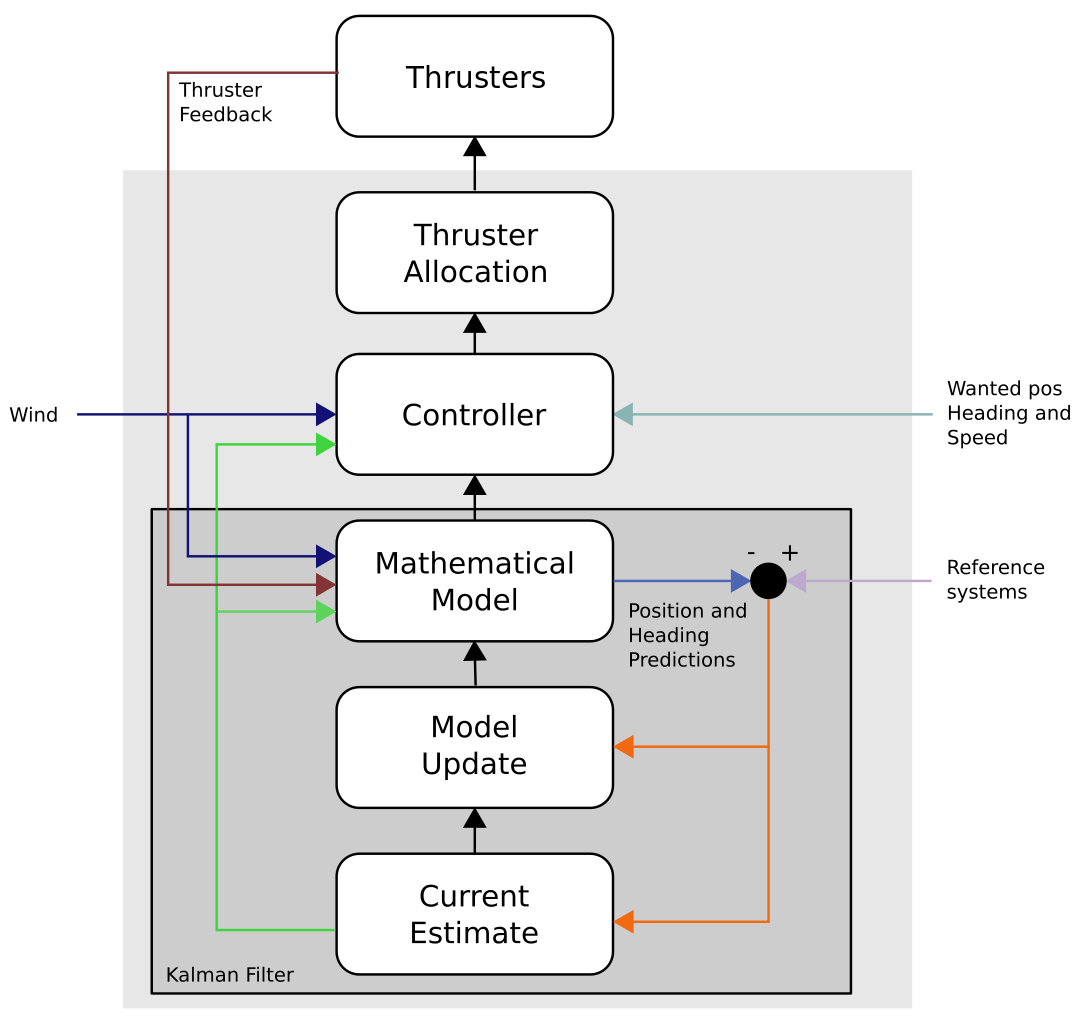
\includegraphics[scale=0.35]{dparchitecture}
	\caption{Model architecture of Dynamic Positioning systems}
	\label{fig:dparchitecture}
\end{figure}


The system contains a \textit{controller} module that influences vessel movements by taking decisions on power allocation for individual vessel thrusters. It takes as input, weather information from wind sensors and current position information from position reference systems. Expected output is to position the vessel at a position and heading preset by the operator. After being initiated, the system determines the difference between current position and desired position. It then attempts to minimize this difference over time. This is done by firing appropriate thrusters into action, producing vessel movements in different directions. 

Environmental forces acting on the vessel during the time though add to the complexity of this operation. The controller then needs to compensate for unpredictable environmental forces as it decides on allocations for individual thrusters.  While the system takes into account wind forces acting on the vessel measured using wind sensors, as shown in \ref{fig:shipforces}, a vessel's position is also affected by ocean currents and waves. Kalman filter is generally used to model the environmental forces. It is an algorithm that uses a series of measurements observed over time, containing statistical noise and other inaccuracies, and produces estimates of unknown variables by using Bayesian inference and estimating a joint probability distribution over the variables for each timeframe. While it tends to be more precise than algorithms based on a single measurement alone, it is a nevertheless a probability based system that produces estimate predictions of changes in environmental forces over time and some uncertainty in predictions can be expected. Although there do not exist rules specifying acceptance criteria for the positioning performance of DP systems, DNVGL guidelines state that "in moderate weather conditions and with a fully operational DP-system the vessel should generally be able to demonstrate position keeping accuracy with a 3 meter radius and $ \pm $ 1\degree of heading." \cite{veritas2011dynamic} 

\todo[inline]{write about accidents that occured. ekofisk etc}

Figure \ref{fig:praxisdp} shows the interface of a typical DP system. A display monitor is used to show various information regarding the vessel and its control systems. Apart from the display, there exists input interface in the form of buttons. They are used to provide information to the system such as desired location and the mode in which it will be used. 

\paragraph{Dynamic Positioning Modes}
Dynamic positioning systems can be commonly operated in different modes. Modes define the type of automatic vessel operation, some of which differ in the amount of automation involved. Following are some common modes of dynamic positioning systems. 

\begin{figure}
	\centering
	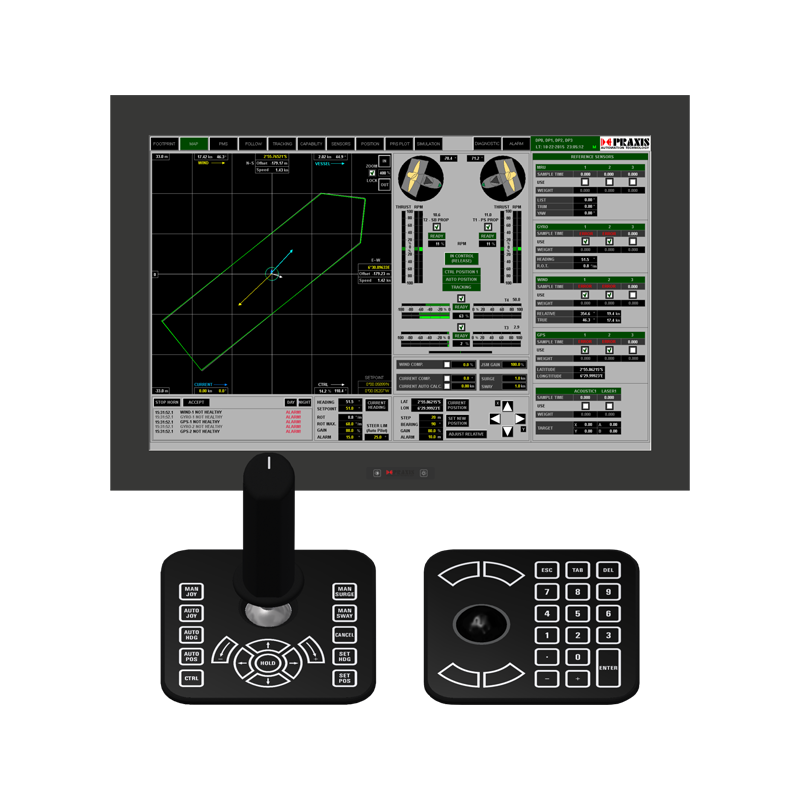
\includegraphics[scale=1]{praxisdp}
	\caption{Typical dynamic positioning console}
	\label{fig:praxisdp}
\end{figure}

\begin{enumerate}

\item \textbf{Joystick}: In this mode, the operator can control the vessel position and heading manually using a joystick. 
\item \textbf{Auto heading}: In this mode, the vessel automatically maintains a preset heading. 
\item \textbf{Auto position}: This mode automatically maintains the vessel's position and heading. 
\item \textbf{Follow target}: Enables the vessel to automatically follow a moving target. 
\item \textbf{Autopilot}: In this mode, the vessel steers automatically to follow a predefined course. 

\end{enumerate}

This is by no means an exhaustive list of DP modes. It can be noted that besides functionality, the modes listed above differ by the level of automation involved in the functionality.  The joystick mode offers the least amount of automation. In this mode, a single lever can be used to control all of the vessel's thrusters at the same time. A large vessel such as a platform supply vessel typically has two azimuth thrusters at the stern-end of the vessel and one at the bow-end. In addition, they also typically have tunnel bow thrusters that can be used to turn the vessel in place. While it is possible to control each of the thrusters individually from the bridge of the vessel for fine-grained control; the joystick mode encapsulates all the thrusters into one control. This allows control of forward, reverse, steering and even sideways motion using just one lever.

%\missingfigure{insert layout of typical PSV thrusters}

\begin{figure}
	\centering
	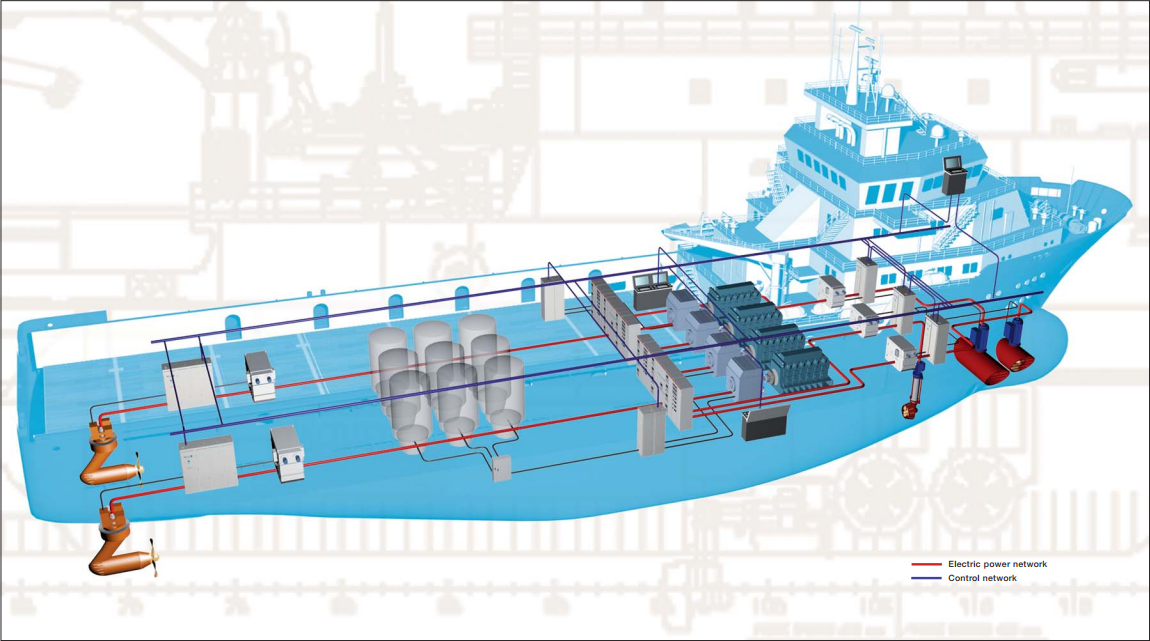
\includegraphics[scale=0.45]{osvlayout}
	\caption{Schematic diagram of the power and control network of a typical offshore supply vessel}
	\label{fig:osvlayout}
\end{figure}

\subsubsection{Manual Handling}
Going by number of total losses occuring per year (refer figure \ref{fig:lossesbyyear}), the safety of vessels world-wide can be said to have improved over the years, particularly the last decade, despite the ever increasing number of sea-faring vessels. Nevertheless, there is a growing concern in the industry regarding overreliance on electronic navigation aids. Studies have found human error to be dominant factor in a significant percentage of the accidents \cite{baker2005accident, hauff2014analysis}. Incidents such as the Norne shuttle tanker's collision with an FPSO on 5 March 2000, Big Orange XVIII's collision with the water injection facility Ekofisk 2/4-W on 8 June 2009 and standby vessel Far Symphony's impact with the mobile installation West Venture on 7 March 2004 are mentioned as cases of shipping incidents that showcase the lack of preparedness among crew members to handle with emergency situations \cite{vinnem2013offshore}.

\begin{figure}
	\centering
	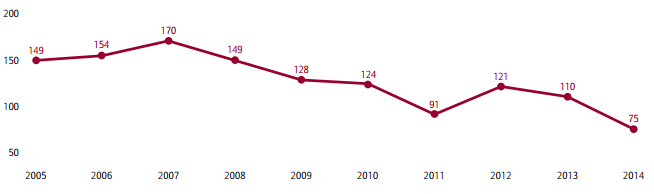
\includegraphics[scale=0.75]{lossesbyyear}
	\caption{Schematic diagram of the power and control network of a typical offshore supply vessel}
	\label{fig:lossesbyyear}
\end{figure}

\section{Operational Demands}

An intuitive understanding of the vessel’s handling is required to manually manoeuvre the vessel. Different vessels exhibit different handling behavior depending on their propulsion technology, steering controls, and, dynamics of the particular vessel, owing to its design. These factors have a combined effect on the handling behavior of the vessel, that is unique to the vessel, or the vessel type in general. Besides, vessels also differ in the way they respond to various weather conditions. 
Gaining a high level of intuitive understanding of the vessel’s motion dynamics comes with extensive practice. A manoeuvre training system should then enable maneuvering practice on the real vessel in real situations.

A clear view of the target object around which the vessel is being maneuvered, provides direct visual feedback of the target’s position relative to the vessel. By looking out the bridge windows, the operator can immediately learn about the progress of the maneuvering operation. Using this information, the operator can make adjustments to the vessel's movement as required.

When maneuvering large vessels, besides the person at the helm, another person usually aids the operation. Standing outside the bridge of the vessel, this person keeps a lookout for the position of the ship, and conveys it to bridge personnel. He also keeps a lookout for traffic and other objects in the vicinity such as navigational aids.

\section{Human Factors Knowledge}
\subsection{Mode Errors}
In context of interface design, mode errors are the errors that occur when a user operates an interface in a manner that is appropriate to a different state of the system than the one it actually is in. When the user forgets the actual state and performs an action appropriate to a different state, the system response is unexpected and usually undesired. A common example of mode errors is the undesired input of capitalised letters on a computer due to caps lock, or the inability to enter numbers using the number pad due to numlock. 

The design of a ship operation training method set in augmented reality needs to take into account the possibility of mode errors resulting from the two realities that are simultaneously at play. A trainee moving a real ship in augmented reality is also moving it in actual reality. Take the example of a training exercise to approach a virtual object out in the open sea. In the course of the exercise, the trainee moves the vessel towards the virtual object in the augmented reality. At the same time, the real vessel is actually moving somewhere out in the open sea. If the bridge equipment is also augmented, the radar would be expected to display an indication of the virtual oil platform. Adding a virtual object to a radar display that already contains information regarding other real objects can be confounding to users. A way to distinctly identify virtual objects should help reduce mode errors but it also hampers immersiveness of the experience. 
It is advised to avoid the possibility of mode errors when possible (citation needed). 

\begin{figure}[ht]
    \centering
    \begin{subfigure}[b]{0.45\textwidth}
        \centering
        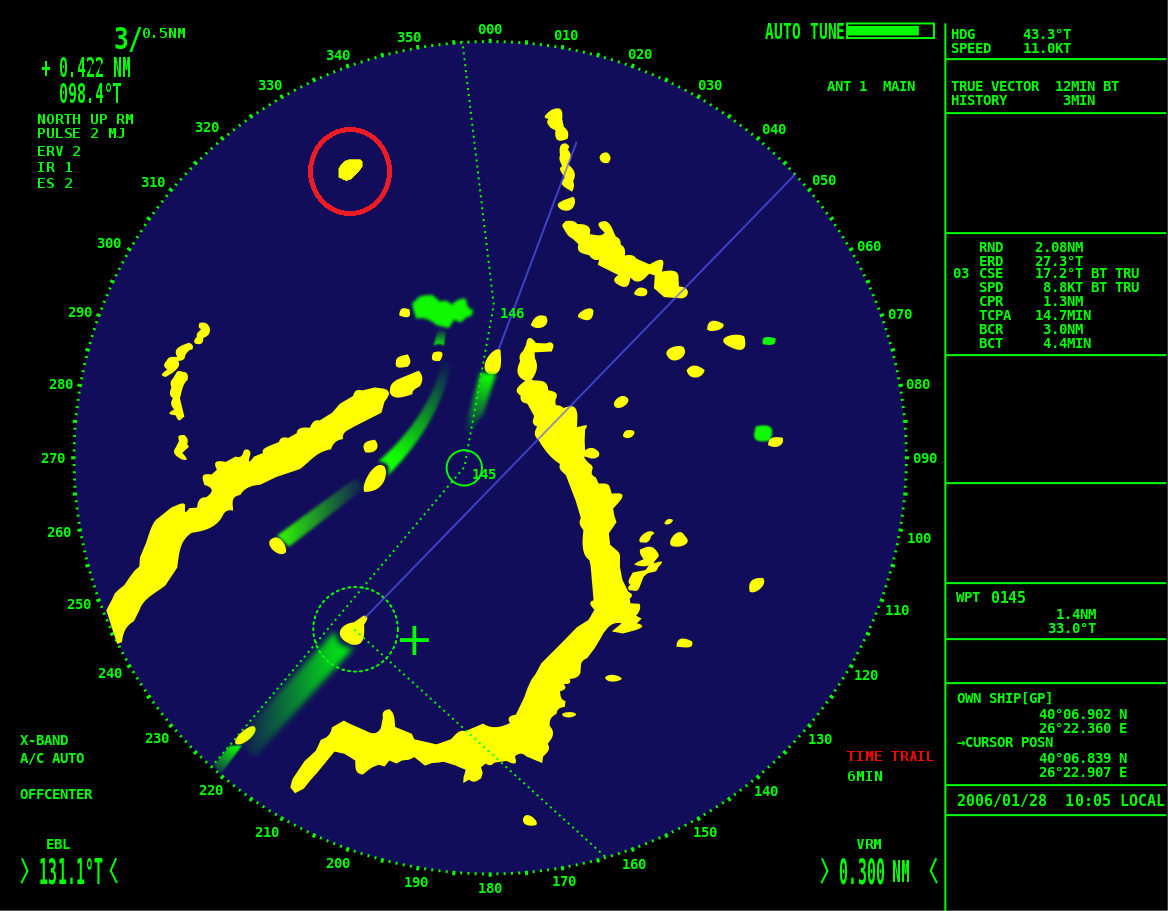
\includegraphics[width=\textwidth]{radarOrig1}
        \caption{No colour differentiation}
        \label{fig:three sin x}
    \end{subfigure}
    \hfill
    \begin{subfigure}[b]{0.45\textwidth}
        \centering
        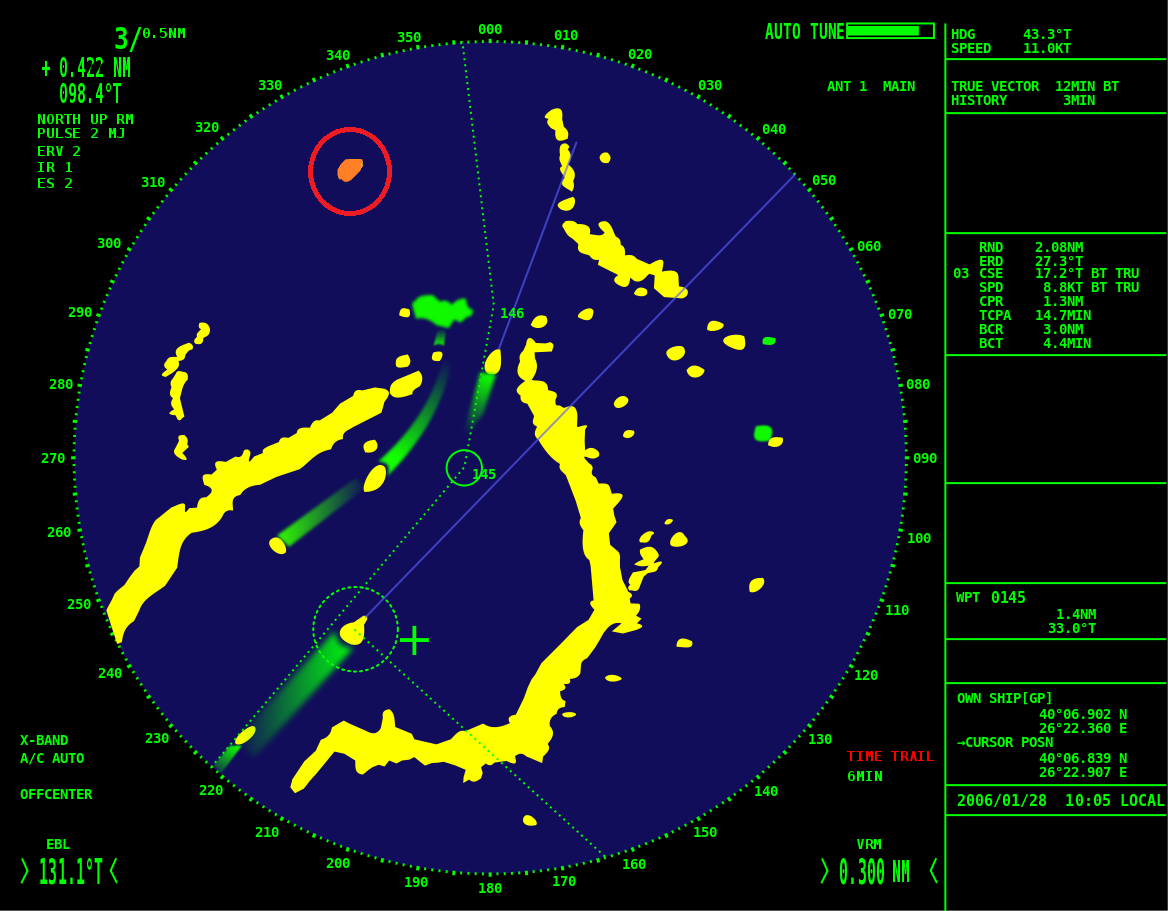
\includegraphics[width=\textwidth]{radarOrig2}
        \caption{Differentiated virtual object}
        \label{fig:five over x}
    \end{subfigure}
    \caption{Display of virtual objects on radar}
    \label{fig:three graphs}
\end{figure}

\section{Envisioned Technology}

An important choice in the design of a new human-computer interface is the technology used to build prototypes, and eventually the end product. For example, devices like keyboard, mouse and trackpad have acted as the standard input interface for personal computers for over 2 decades now, while computer monitors in the form of CRT, LCD and TFT displays have formed the output interface. Not unlike television monitors, computer monitors were initially used for purposes of data processing before being used for entertainment purposes such as gaming and media streaming. With the evolution of computing technology from large machines driven by punch cards and that filled up entire rooms to the personal computer form has coincided with their ubiquitous use in the modern world influencing the manner in which most white collar jobs today are carried out. 

\todo[inline]{consider relevance of following paragraph to this section}
Computers had a significant impact on the maritime industry. Where naval architecture was traditionally a craft with little scientific information to back designs, modern computers enabled computing power to be leveraged to predict performance. Modern ship designs make use of tools that have been developed to assess static and dynamic stability, water resistance, for hull development and structural analysis. Among other uses, maritime industry found use for computers as devices that could be used for the simulation of movements of vessels on sea. In a gaming-like use case, computers are used to run ship simulation software for educational purposes. These programs can be used to control virtual ships in virtual marine environments. Some setups involve actual bridge equipment to input commands to the program, making the experience more real-like. An array of monitors are used for display. Backed by computer graphics and models of sea, vessel and other objects, the simulation software is supposed to create the perception of being inside a real vessel. It is now standard practice to undergo training using simulators in the maritime industry. 

Figure \ref{fig:dpoflowchart} shows the certification process required to be a qualified dynamic positioning operator. One starts with a classroom-based induction course that provides basic knowledge of the principles and practical use of DP. After such a course, the trainee is expected to be familiar with the components of a DP system, concept of redundancy that separate different classes of DP systems, its modes of operation and limitations. Thereafter the trainee goes on to acquire watchkeeping experience onboard real vessels with DP. This watchkeeping exercise takes place for a relatively short period of time where the trainee is familiarised with DP equipments onboard the vessel and gets to witness operations. This is followed by a simulator-based course where the trainee gets practical experience operating DP systems in onshore simulation centers.  

\begin{figure}
	\centering
	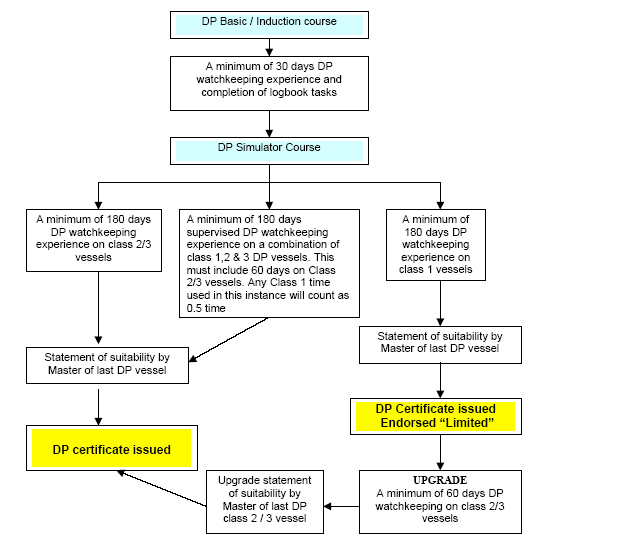
\includegraphics[scale=0.75]{dpoflowchart}
	\caption{Flowchart of nautical institute Dynamic positioning certificaiton scheme}
	\label{fig:dpoflowchart}
\end{figure}



on-board training method is the hardware technology that will be used for the human-computer interface.

\subsection{Display Technology for Mixed Reality}

This section talks about creation of visual perception of mixed reality using digital display technology. 
\subsubsection{Photorealism}

\begin{table}[h]
\centering
\caption{Levels of photorealism}
\label{tab:trainingoptions}
\begin{tabular}{@{}p{2cm}p{10cm}@{}}
\toprule
\multicolumn{1}{c}{\textbf{Classification}} & \multicolumn{1}{p{10cm}}{\textbf{Reasoning}} \\ 
\hline
High & \vspace{-2mm} \begin{enumerate}[leftmargin=*,topsep=0pt,partopsep=0pt,align=left,itemsep=0.05cm]
\item Presentation of occlusion, a basic depth cue, is necessary to induce sense of depth in the augmented scene
\item Wide field of view is required to create illusion of large object being nearby.	
\item  Virtual object is the main focus in the scene and, inconsistency in 3D view of augmented reality can hamper task performance from visual fatigue due to accomodation-vergence conflict.
\end{enumerate}
\vspace{-\baselineskip}\\
\hline
Medium & \vspace{-2mm} \begin{enumerate}[leftmargin=*,topsep=0pt,partopsep=0pt,align=left,itemsep=0.05cm]
\item Occlusion is useful to induce depth in the scene, but some amount transparency can be tolerated.
\item  Lack of wide field of view does not affect task performance. 
\item  Inconsistency in 3D view does not easily amount to visual fatigue as virtual object is not the user's main object of focus in the augmented scene.
\end{enumerate}
\vspace{-\baselineskip}\\
\hline
Low & \vspace{-2mm} \begin{enumerate}[leftmargin=*,topsep=0pt,partopsep=0pt,align=left,itemsep=0.05cm]
\item Depth cues in the scene are not necessary for purposes of the training.
\item Wide field of view is not required for effective task performance.
\item Inconsistency in 3D view does not easily amount to visual fatigue as virtual object is not the user's main object of focus in the augmented scene
\end{enumerate}
\vspace{-\baselineskip}\\
\bottomrule
\end{tabular}
\end{table}

\subsubsection{Categories of Mixed Reality Display}
\paragraph{Optical See-Through Head-Mounted Display}

\paragraph{Video See-Through Head-Mounted Display}

\paragraph{Spatial Augmented Reality}

\subsection{Ship Instrument Augmentation}

\subsubsection{Bridge Instrumentation}

\subsubsection{Tracking Requirements}

\paragraph{In-out vs out-in tracking}

\paragraph{Fiducial Markers}
